\chapter{Objetivos}\label{cap:objetivos}

\section{Problema a resolver}

Como se ha introducido en el Capítulo~\ref{cap:introduccion}, el objetivo principal de este TFG es dotar al humanoide NAO de una capa completa de movimientos y locomoción, para luego programar una aplicación que empleará este robot educativo en el ámbito de la robótica de servicios. Esta aplicación servirá además de validación para demostrar que dicha capa de movimiento es funcional e intuitiva de utilizar.

Sin embargo, este objetivo es muy general y amplio, así que lo mejor es dividirlo en subobjetivos, que se detallan a continuación.

\begin{itemize}
    \item \textit{Subobjetivo 1}: Como primer subobjetivo tenemos el ser capaces de crear patrones fijos de movimiento y que NAO pueda replicarlos fielmente y con los menores errores posibles.
    \item \textit{Subobjetivo 2}: El segundo subobjetivo de este proyecto es dotar al humanoide de la capacidad de parametrizar sus movimientos y  poder ofrecer modos de caminar distintos y con la velocidad variable, obteniendo así movimientos continuos parametrizables. Estos movimientos deben encapsularse en una librería para que su uso sea más sencillo y directo. Dicha librería contendrá además toda la funcionalidad de ROS2 y los patrones fijos ofrecidos por el robot (desarollados para el subobjetivo 1), para que así sea una biblioteca utilizable por cualquier usuario de manera sencilla.
    \item \textit{Subobjetivo 3}: Como tercer y último subobjetivo, tenemos el desarrollar una aplicación que sirva de demostradora de la potencia de dicha libería, haciendo que el robot preste servicio en un invernadero.

    El servicio que debe ofrecer es similar al visto en el robot Digit, esto es, mover una caja de un lugar de origen a uno de destino, pero, en lugar de en un almacén, se hará en un invernadero para dar más identidad y originalidad al proyecto.
\end{itemize}

\section{Metodología}

Para alcanzar los subobjetivos planteados y, en última instancia, cumplir con el objetivo principal del proyecto, se ha optado por adoptar la metodología \textit{Scrum} como marco de trabajo. Esta elección responde a la necesidad de mantener una dinámica de desarrollo iterativa y adaptable (Esquema del funcionamiento de esta metodología en la \autoref{fig:scrum}). 

\begin{figure}[H]
    \centering
    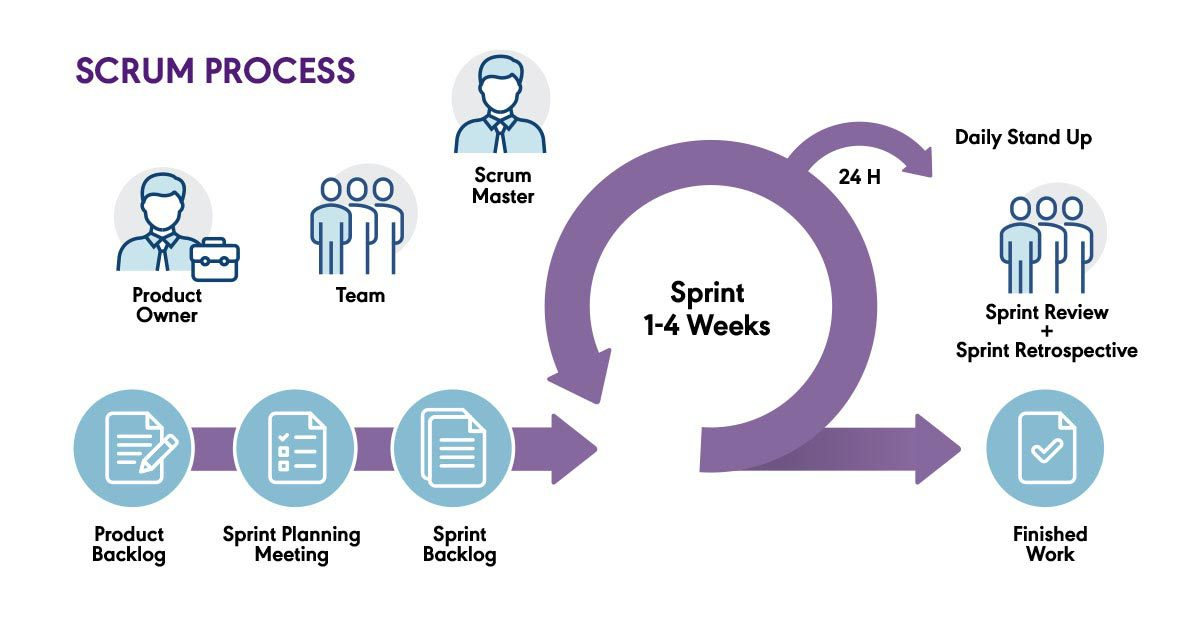
\includegraphics[width=1\textwidth]{figures/cap_2/scrum.jpg}
    \caption{Esquema del funcionamiento de la metodología \textit{Scrum}}
    \label{fig:scrum}
\end{figure}

En este contexto, se han establecido reuniones semanales con el tutor del proyecto, que cumplen la función de revisiones periódicas del progreso similares a las \textit{Sprint Reviews}, ya que, durante estas sesiones, se evalúan los avances logrados en la última iteración y se definen de manera colaborativa los siguientes pasos a seguir. Este enfoque permite ajustar la planificación de forma continua en función de los resultados obtenidos, fomentar la mejora progresiva del proyecto, y asegurar que cada etapa del desarrollo esté alineada con los objetivos generales. De esta manera, se garantiza un proceso flexible, enfocado en la entrega constante de valor y la toma de decisiones informadas a lo largo del ciclo de desarrollo.

En resumen, la metodología que se ha aplicado estaba basada en \textit{sprints} de \textit{Scrum} semanales los cuales iba marcando mi tutor, en función a los objetivos cumplidos del sprint anterior.

\subsection{Plan de trabajo}

El primer \textit{sprint} de trabajo fue elegir una plataforma para alojar el proyecto y facilitar el seguimiento del mismo.

Para cumplir con eso, se ha decidido alojar el código fuente generado en un repositorio de GitHub\footnote{\url{https://github.com/}}, plataforma que ayuda a los desarrolladores a almacenar y gestionar su código, así como a rastrear y controlar los cambios en él, lo que lo convierte en la plataforma de control de versiones preferida a la hora de desarrollar proyectos grandes, como es el caso de este TFG.

Que sea un sistema de control de versiones nos ayuda a tener registradas todas y cada una de las versiones del proyecto, pudiendo volver a una versión anterior o seguir avanzando a placer. Esto es de gran ayuda por si es necesario volver a una versión anterior por cualquier razón.

El repositorio dónde se aloja este proyecto\footnote{\url{https://github.com/RoboticsLabURJC/2024-tfg-eva-fernandez}} sigue la siguiente estructura:

\begin{itemize}
    \item \textit{Directorio CoordMoves}: Es en este directorio donde se aloja el proyecto completo, códigos, modelos, mundos, este documento, etc.
    \item \textit{Directorio pruebas}: En este directorio fue donde se trabajó durante la fase experimental del proyecto, con todo lo que eso conlleva. 
    \item \textit{Directorio docs}: Directorio dónde se aloja un blog de seguimiento semanal del proyecto. Esto se tratará con profundidad más adelante.
    \item Fichero \textit{README.md}: Un fichero en el que se describe de forma resumida todo el proyecto, ya que éste es público.
\end{itemize}

También se ha decidido utilizar Github Pages\footnote{\url{https://pages.github.com/}}, un servicio de alojamiento de sitios estáticos que toma archivos HTML, CSS y JavaScript directamente de un repositorio en GitHub, los ejecuta opcionalmente mediante un proceso de compilación y publica un sitio web. Ha sido utilizado en el proyecto para llevar un blog semanal\footnote{\url{https://roboticslaburjc.github.io/2024-tfg-eva-fernandez/}}, en el que se comentan avances, percances o ideas que han surgido durante el desarrollo del proyecto, desde su inicio, hasta su fin.

Este blog es una forma muy potente de documentar el proceso de desarrollo y poder seguir el esquema \textit{Scrum}, ya que, no sólo es interesante para ver cómo se ha hecho o qué se ha hecho, si no que ha servido de mucha ayuda para que mi tutor tuviera un seguimiento más rígido del proceso y se pudieran abarcar todas las cuestiones y avances realizados en las reuniones.

Los sprints siguientes fueron más variados, cómo buscar un modelo, prepararlo junto a un primer mundo, descubrir cómo controlar este modelo con ROS2, etc. Lo que nos dejó 3 fases principales a la hora del desarrollo:

\begin{itemize}
    \item \textit{Fase 1}: Preparación del modelo y un mundo vacío
    \item \textit{Fase 2}: Desarrollo de un intérprete de movimientos y un editor
    \item \textit{Fase 3}: Implementación de la librería y llenado del mundo
    \item \textit{Fase 4}: Desarrollo de la aplicación
\end{itemize}